\listfiles
\documentclass[a4paper, oneside]{report}

\usepackage[utf8]{inputenc}
\usepackage[francais]{babel}

\usepackage{amssymb}

\usepackage[pdftex]{graphicx}
\usepackage{graphics}

\usepackage[top=3cm, bottom=2cm, left=3cm, right=2cm]{geometry}

\usepackage{multirow}
\usepackage{tabularx}

\usepackage{listings} % a inclure pour la fonction listing
\usepackage{color} % on en a besoin pour utiliser les couleurs
\definecolor{grey}{rgb}{0.95,0.95,0.95} % on definit la couleur grise (c'est un gris tres clair)
		
\usepackage{float}

\renewcommand{\floatpagefraction}{.9} 
%utilisee avec la commande :
\renewcommand{\textfraction}{.1}
%permet de dire que le texte peut n'occuper que 10% d'une
%page, et donc que des flottants peuvent occuper les 90% restant.


%Il y a d'autres parametres interessants :
\setcounter{totalnumber}{4} 
\setcounter{secnumdepth}{3}
%qui determine le nombre de flottants autorises par page,
\renewcommand{\topfraction}{.8}
\renewcommand{\bottomfraction}{.8}

\lstset{numbers=left, tabsize=2, frame=single, breaklines=true, basicstyle=\ttfamily, numberstyle=\tiny\ttfamily, framexleftmargin=13mm, backgroundcolor=\color{grey}, xleftmargin=12mm}

% titre du document
\title{IN41 \\Syst\`emes Lin\'eaires Continus \& Filtrage Analogique \\TP4 : Filtrage}
% auteur du document
\author{Maxime Ripard}

\begin{document}
  \maketitle
  \newpage{}
  \tableofcontents
  \newpage{}

  \chapter{Multiplexage d\'emultiplexage}
    \section{D\'efinition}
 
Le multiplexage consiste \`a faire passer plusieurs informations \`a travers un seul support de transmission. On peut trouver deux types de multiplexage : le multiplexage fr\'equentiel et le multiplexage temporel.\\
Alors que le premier s\'epare les signaux dans des gammes de fr\'equences diff\'erentes, le multiplexage temporel alterne lui \'`a haute fr\'equence les diff\'erents signaux \`a la mani\`ere d'un commutateur.\\
Le d\'emultiplexage est l'op\'eration inverse qui consiste \`a obtenir les diff\'erents signaux \`a partir du signal provenant du canal de transmission.\\

    \section{Exemples d'applications}
  
  Le multiplexage temporel peut \^etre utilis\'e pour pouvoir utiliser un convertisseur analogique/num\'erique ou num\'erique/analogique avec plusieurs entr\'ees et sorties en simultan\'ee.\\
Il est \'egalement utilis\'e par les transmissions informatiques (USB, IEEE 1394, SSA, Serial ATA) et dans la transmission de cha\^ines de t\'el\'evision num\'erique.\\
Il est aussi couramment utilis\'e dans l'industrie automobile concernant les cablages des v\'ehicules. \\

Le multiplexage fr\'equentiel est quant \`a lui utilis\'e dans l'utilisation de la capacit\'e de transmission des fibres optiques ou pour le t\'el\'ephone, par exemple pour faire passer la voix et l'ADSL dans la m\^eme ligne t\'el\'ephonique, sans collision, gr\^ace \`a un filtre.

 
 \chapter{Multiplexage}
 
\begin{lstlisting}
t=[0:1/fs:1];
x1 = sin(2*pi()*5*t);
x2 = sin(2*pi()*4*5*t);
x3 = sin(2*pi()*7*5*t);
x = x1 + x2 + x3;

figure(1)
plot(t,x,'b',t,x1,'r:',t,x2,'m:',t,x3,'k:')
grid
axis([0 0.2 -3 3])
title('Signal x(t)')
xlabel('Temps t')
ylabel('Amplitude') 
legend('x=x1+x2+x3','x1=sin(2*pi*5*t)','x2=sin(2*pi*20*t)','x3=sin(2*pi*35*t)')
\end{lstlisting}

 \begin{figure}[h]
 \centering
 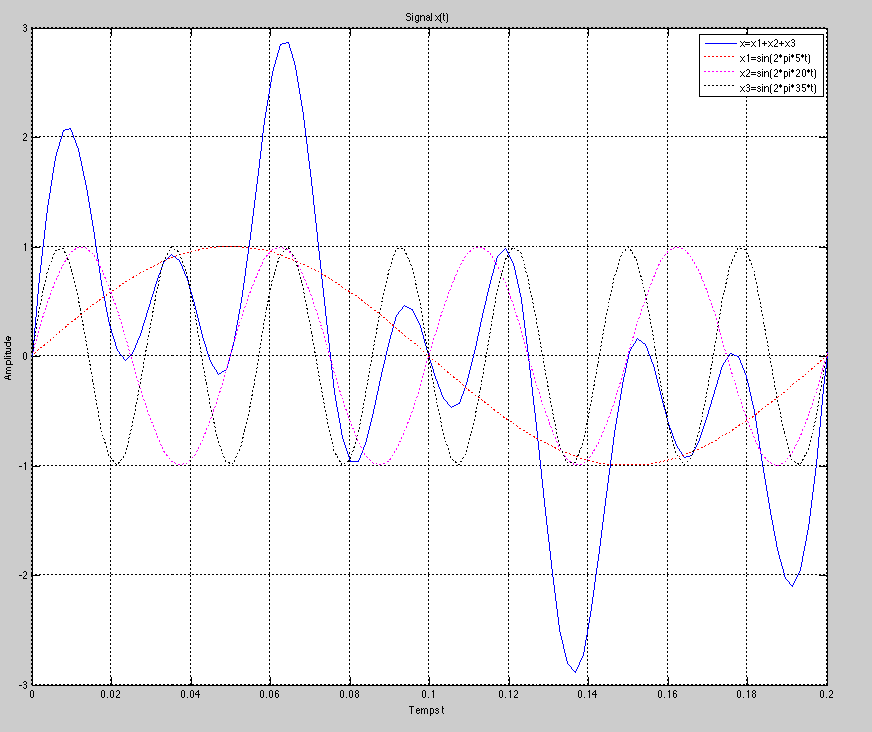
\includegraphics[scale=0.5]{images/xt.png}
 \caption{D\'ecomposition en S\'erie de Fourier}
 \end{figure}
 	  
  \chapter{D\'emultiplexage avec le filtre de Chebyshef}
 		
 \begin{figure}[h]
 \centering
 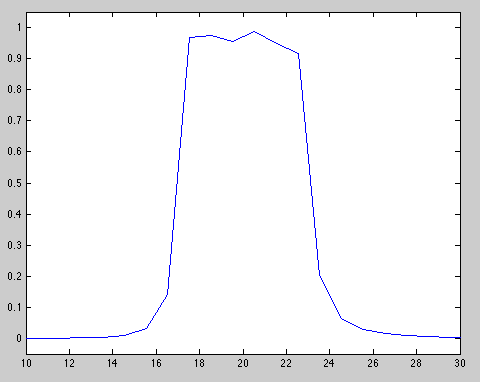
\includegraphics[scale=0.8]{images/cheby.png}
 \caption{Valeur absolue du filtre de Chebyshef}
 \end{figure}
 
 
On applique le filtre de Chebyshef sur notre signal x(t), somme de 3 signaux de diverses fr\'equences.\\
Le signal en sortie est de la forme $|sin(2\pi f2t)|$.
De plus, le signal en entr\'ee X(f) se compose de 3 raies correspondant aux fr\'equences des 3 signaux somm\'es de x(t).\\

Dans le cas de notre filtre passe-bande appliqu\'e au signal x(t) nous allons conserver les fr\'equences comprises dans la bande-passante du filtre, c'est-\`a-dire dans l'intervalle [17,5;22,5] ici puisque nous avons une BP=5Hz et une Fc=20Hz.\\
Le filtre va donc rejeter les raies \`a 5Hz et \`a 35Hz correspondant aux signaux x1(t) et x3(t). En ne conservant que la raie \`a 20Hz nous obtenons le signal x2(t).\\

C'est donc bien un d\'emultiplexage qui est effectu\'e ici bien que le signal x2(t) r\'ecup\'er\'e ne soit pas parfaitement reconstitu\'e \`a cause de l'ordre du filtre qui n'est pas infini. Le filtre de Chebyshef utilis\'e ici n'est pas id\'eal mais s'en approche beaucoup.\\

L'utilisation du filtre de Chebyshef nous permet donc de ne garder qu'un signal sur ceux multiplex\'es au d\'epart et de s'approcher de l'application d'un filtre id\'eal \`a notre signal en entr\ 'ee.\\

 \begin{figure}[h]
 \centering
 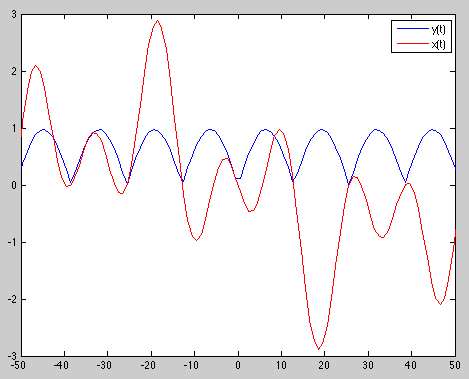
\includegraphics[scale=0.8]{images/fourier_inv.png}
 \caption{Filtre sur le signal x(t) avec Fc=20Hz}
 \end{figure}
 
 Pour r\'ecup\'erer un autre signal il suffit de changer la fr\'equence de coupure sur sa fr\'equence. Ainsi pour r\'ecup\'erer le signal x3(t) il suffit de placer la fr\'equence de coupure du filtre \`a 35Hz et restreindre la bande-passante afin de ne pas r\'ecuperer un autre signal qui serait proche en fr\'equence.\\
 On a donc appliqu\'e ici le m\^eme filtre de Chebyshef avec Fc=35Hz.\\
 Si on voulait r\'ecup\'erer x1(t) il suffirait de proc\'eder de la m\^eme mani\`ere et de placer la fr\'equence de coupure \`a 5Hz.
 
 \begin{figure}[h]
 \centering
 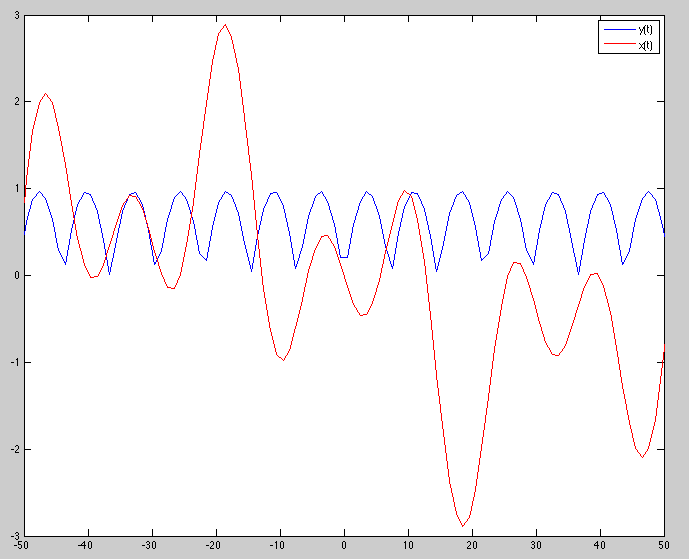
\includegraphics[scale=0.65]{images/fourier_inv35.png}
 \caption{Filtre sur le signal x(t) avec Fc=35Hz}
 \end{figure}
\newpage
Un ordre plus \'elev\'e nous montre des fronts de mont\'ee et de descente de la porte de plus en plus marqu\'e au fur et \`a mesure que l'ordre du filtre augmente. Ce qui prouve bien que les filtres id\'eaux sont des filtres d'ordres infinis.
Le signal reconstruit sera de plus beaucoup plus pr\'ecis et similaire au signal de d\'epart en augmentant l'ordre.

\begin{figure}[h]
\centering
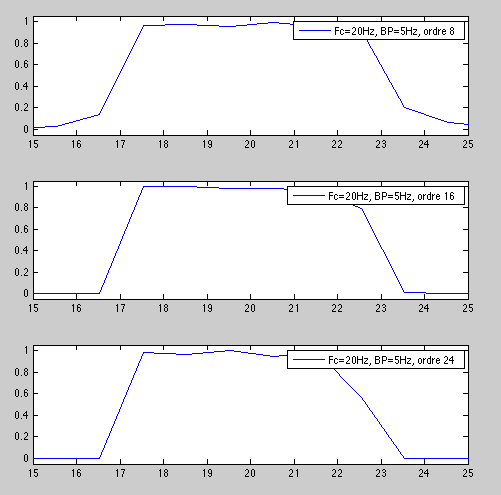
\includegraphics[scale=0.8]{images/cheb_divers.png}
\caption{Application de 3 ordres diff\'erents au filtre}
\end{figure}

 
  \chapter{D\'emultiplexage avec un filtre de Butterworth}
 
 \begin{figure}[h]
 \centering
 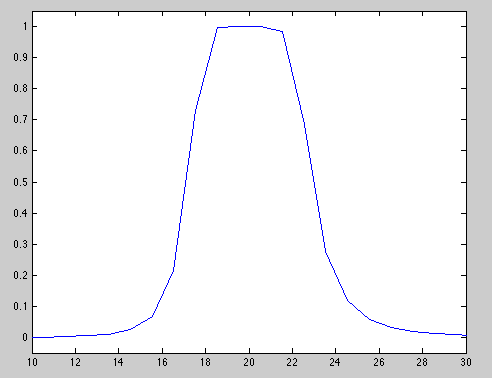
\includegraphics[scale=0.8]{images/butter.png}
 \caption{Valeur absolue du filtre de Butterworth pour un ordre 8}
 \end{figure}
  
 En comparant le filtre de Chebyshef avec le filtre de Butterworth on remarque que le filtre de Chebyshef semble plus pr\'ecis lorsque l'ordre est grand. D'un autre c\^ot\'e, le filtre de Butterworth n'ondule pas dans l'intervalle de la bande-passante.\\
 Quel que soit le filtre utilis\'e, pour se rapprocher d'un filtre id\'eal il faut prendre un ordre \'elev\'e.
 \newpage
  
 \begin{figure}[h]
 \centering
 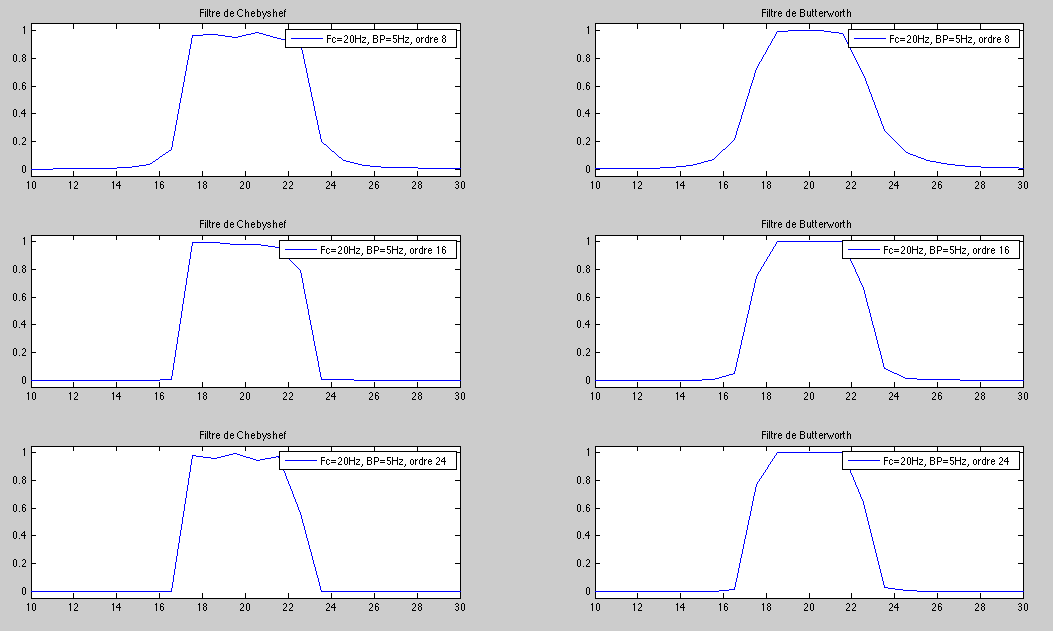
\includegraphics[scale=0.45]{images/butt_cheb.png}
 \caption{Comparaison du filtre de Chebyshef avec le filtre de Butterworth}
 \end{figure}

On remarque donc que plus l'ordre est \'elev\'e, plus le filtre reconstruit le signal \`a l'identique de celui en entr\'ee. Toutefois, le filtre de Chebyshef semble plus pr\'ecis pour un ordre \'egal \`a 16 m\^eme si pour un ordre sup\'erieur on se rapproche d'un r\'esultat identique.
  
\begin{figure}[h]
\centering
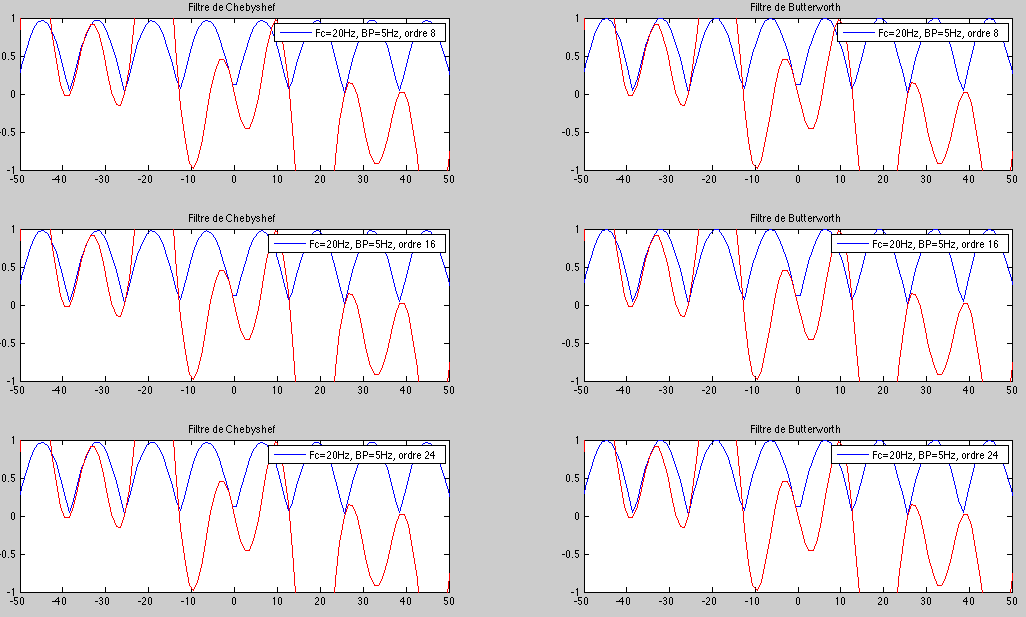
\includegraphics[scale=0.4]{images/signal_butt_cheb.png}
\caption{Comparaison de la reconstitution du signal selon les 2 filtres}
\end{figure}
 	
 \chapter{Bilan}

Pour conclure, afin de r\'ealiser un d\'emultiplexage quasi id\'eal, il faut appliquer un filtre ayant un ordre le plus \'elev\'e possible sur le signal.
Il faut n\'eanmoins tenir compte du fait que plus l'ordre sera grand, plus le filtre sera complexe et donc moins r\'ealisable.\\

C'est pourquoi, il faudrait privil\'egier l'utilisation du filtre de Chebyshef par rapport au filtre de Butterworth car il nous fournit de meilleurs r\'esultats pour un ordre moyen tout en gardant une bonne pr\'ecision.\\

Toutefois, du fait de l'ondulation dans la bande-passante, pour conserver les informations sur l'amplitude du signal, on privil\'egiera le filtre de Butterworth.
Cela d\'ependra donc de l'application que l'on aura \`a effectuer.
  
\end{document}